\documentclass[]{article}

\usepackage{cite}
\usepackage{hyperref}
\usepackage[a4paper, total={6in, 10in}]{geometry}
\usepackage{graphicx}
\graphicspath{ {images/} }



%opening
\title{Peerster - NoTrust\\
Team NoTrust}
\author{Raja Soufi, Pierre Thevenet}

\begin{document}

\maketitle

\begin{abstract}
The goal of our project is to extend Peerster's file sharing to include a reputation system, and include authenticity, confidentiality and integrity for files and messages. This will allow safer file transfer, and a fairer network.
\end{abstract}

\section{Goals and Functionalities}

\subsection{Authenticity, Integrity, Confidentiality and Web-of-Trust}

\subsubsection{Authenticity and Integrity in File Sharing}
\label{sec:goals-funcs-auth-integrity}
One of the goal is to add a way to verify the origin of a file. That is if a peer A receives a file from origin B, A can verify if the true origin is indeed A. If it is, then it can accept the file, and if not, decide to discard the file and decrease the reputation of the sender (see \ref{sec:sig-based-rep}). \newline

In the user's perspective, the received files will only be origin validated files, so the user does not need to think if the file received has been modified from someone else than the origin. The verification process is not visible.
Integrity will be implemented with authenticity.

\subsubsection{Confidentiality}
In the user's perspective, this will allow the possibility to send encrypted files and messages to a (single) known destination. Because the peerster network is open to eavesdroppers, this will offer confidentiality in one-to-one communication.

\subsubsection{Decentralized Key Sharing, Web of Trust}
The previous functionalities are implemented using public key cryptography. Usually the public keys are shared using a centralized PKI (Public Key Infrastructure), but our project will avoid this and implement a decentralized way to distribute public keys, based on the PGP "Web of Trust" model \cite{abdul1997pgp}.

Once the public keys are obtained, the previous functionalities (CIA) are straightforward, therefore this is one of the main goals of our project, with the reputation system.

Our system will build a table of relation between peers and public key, and assign a trust level to each relation, representing the confidence that a particular public key belongs to a particular peer.

In summary our project also consist in a solution to the key validation and distribution problem. 

This enables all benefits from having public keys (e.g. authenticity, confidentiality...), while not relying on trusting a common authority. \newline

In the user's perspective, this way of sharing public keys will not be visible, for the sake of simplicity. However we can imagine an extension in which the trust put in the obtained public keys also depends on the user decision, for example while receiving a suspicious message, the user can decide to distrust the public key associated with the origin of the message.

\subsection{Reputation}
The goal of having a reputation system in our implementation of Peerster is to improve the efficiency and security of the network.
Every peer A will compute a reputation for every other peer B based on three things:

\begin{itemize}
\item A's interactions with B
\item The communicated reputation of B from other peers, weighted by those other peers' reputations relative to A
\item The respective difference between the reputations of other peers communicated by B and those previously computed by A
\end{itemize}

Two types of reputation are computed for each peer. These are described below.

\subsubsection{Signature-Based Reputation}
\label{sec:sig-based-rep}
Every time A receives signed data originating from C delivered by B (note that B and C might be the same peer), A can check if the data delivered by B actually comes from C by means of Public Key Cryptography (as seen in \ref{sec:goals-funcs-auth-integrity}).
\\\\
If the data turns out to be authentic, then A will increase B's reputation, otherwise A will decrease it.
The amount by which A modifies B's reputation depends on the confidence level of C's public key that A holds, i.e. the degree to which we are confident that the public key we think is that of C is indeed that of C (see \ref{sec:related-work-wot}).

\subsubsection{Contribution-Based Reputation}
This type of reputation represents how much data B has delivered to A, relative to the total amount of data exchanged between the two.
Yet, more importance will be given to more recent interactions, as we will see in more detail in \ref{sec:background}.
\\\\
For this, A will recompute this type of reputation after every interaction with B based on the history of data flow between them.
This means that in a situation where both peers send data to each other in equal amounts, each of them will have a maximal reputation for the other, whereas in a situation where A sends much more data to B than the other way around, B will have a high reputation for A and A will have a low reputation for B.

\section{Related Work}

\subsection{TODO: Choose a title for this subsection}

\subsubsection{Confidentiality, Authenticity and Integrity}
This is a common problem, and solved using cryptography. Since in peerster we do not have a confidential channel to share a common key, we consider only public key cryptography. Two main solutions are RSA \cite{RFC8017} and elliptic curve cryptography (ECC). While ECC may be more promising, RSA is more reviewed.

\subsubsection{Decentralized PKI}
Decentralized PKIs already exist, and the main goal for them is to redistribute the roles of the certificate authorities in the common centralized PKI approach, and usually this mean not storing all public keys at the same place, and trusting the system. KeyChains \cite{morselli2006keychains} and \cite{aberer2005decentralised} are models for a decentralized PKI, the database of public keys are distributed which implies that a peer does not have every public keys, and that the retrieving of keys need more time than storing all keys in each system.

Implementing this in Peerster does not seem necessary, since every peer eventually save the entire set of active peers in the network (due to the specification). Our approach is to collect and save public keys for peers for each peerster client (total decentralization). Therefore this solution will save time for public key lookup, at the cost of storage.

\subsubsection{Web of Trust}
\label{sec:related-work-wot}

The PGP Web of Trust Model \cite{abdul1997pgp} is a way to collect public keys using a social network, usually done in real life. For example, B signs the key of C, and gives the key to A, if A trusts B (which defines B as an "introducer"), A can trust that the given key indeed belong to C, and A can then signs the key of C. 

In Peerster we would want it to be automated, which is not the case in the common PGP model. 

One of the key point of the model is the notion of trustworthiness of certificates and introducers. The trust of a certificate or introducer is decided by the user for each case, in Peerster we want it to be done automatically using the reputation and length of the certificate chain named "key ring" (see Fig. \ref{fig:pgp-key-ring}).

In the PGP model the level of trust is discrete (e.g. 'marginal', 'complete', 'untrustworthy' ...) but the meaning of this levels are not explicit and left for interpretation. We will therefore extend this model with a level of trust representing a 'probability' of confidence in the association key-peer. This idea is described in \cite{haenni2007new}, which is a natural extension to the PGP model and seems reasonable.
A bad aspect for this idea is the need for a threshold for discarding keys with a trust level too low.

\begin{figure}[h]
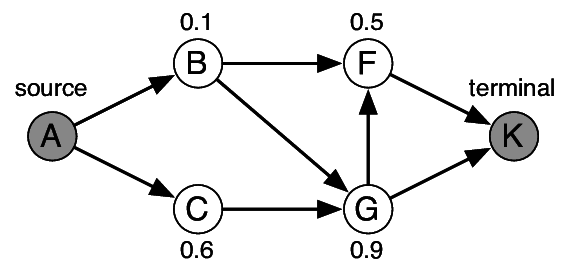
\includegraphics{pgp-key-ring}
\centering
\caption{Example of a PGP Key Ring}
\label{fig:pgp-key-ring}
Source : \cite{haenni2007new}

Here each vertex is a peer, and each edge Y $\rightarrow$ Z means that Y signed the key for Z.
Each figure associated with vertex Z  correspond to the trust level given in the public key, we will name it the probability of Z, $Pr(Z)$.
\end{figure}

\subsection{Reputation}
This is also a common problem, and different variations of a common approach have been studied in order to manage reputation in a distributed system while minimizing the possibilities for malicious peers to abuse the reputation system in order to gain reputation and do malicious activity.
\\
For instance, \ref{gupta2003reputation} computes a global reputation for each peer, which uses local reputation values assigned to it by other peers, weighted by those peers' global reputations.
\ref{despotovic2006p2p} takes a similar approach but computes a trustworthiness of a node by doing a weighted average of the experiences of the nodes that interacted with that node.
Another interesting approach is that of \ref{zhou2007powertrust}, in which each node is rated with a global reputation

\section{Background}
\label{sec:background}

\subsection{Cryptography}
Since our project will be written in go, we will use standard cryptographic libraries for go. We will use RSA \cite{RFC8017}.

\subsection{Web of Trust}
\label{sec:web-of-trust-spec}
We will implement the idea of \cite{haenni2007new}.

\subsubsection{Algorithm}
In details, consider the network in Fig.\ref{fig:pgp-key-ring}. For validating the public key of K, we follow the steps :

1. Compute the shortest paths from A to K \newline
Here the shortest paths are $paths = \{(A,B,F,K), (A,B,G,K), (A,C,G,K)\}$

2. Then compute the "probability" $p$ of the set of paths : \newline
Define, for distinct peers $A_1,...,A_n$ and path $path = (A_1,...,A_n)$, $Pr(path) = \prod_{i = 1}^{n} Pr(A_i)$ \newline
$Pr(paths)$ is computed using the inclusion exclusion formula over the shortest paths. \newline
Here $p = 0.581$

3. If $p > \lambda$ accept the key, else reject it. \newline
Here, if $\lambda = 0.6$, reject the key : the certificate chain may be too long, or the reputation of the peers too low.

\subsubsection{Parameters}
\label{sec:parameters}
$\lambda$ is the acceptance threshold. We will fix it for simplicity. \newline
The 'probabilities' assigned to each peers are computed using the reputation system and the distance from the source in the graph. We will use $min(rep_A, \frac{1}{d})$ as the probability of $A$, where $rep_A$ is the current reputation of $A$ and $d$ is the distance from this peer in the key ring. This way we enforce the distance and the reputation to be acceptable.

\subsubsection{Start}
At first, a peer needs trusted peers to start collecting keys, this peers will be called "first introducers". They need to be given at startup, along with their public key (to effectively trust them).

\section{Design and Architecture}

\subsection{Systems}
Our system can be easily devided into two different but interconnected systems : the Reputation System (RS) and the Web of Trust system (WTS). \newline
Figure \ref{fig:no-trust-arch} illustrates the overall structure of the system and the interactions between the two subsystems.

\begin{figure}[h]
	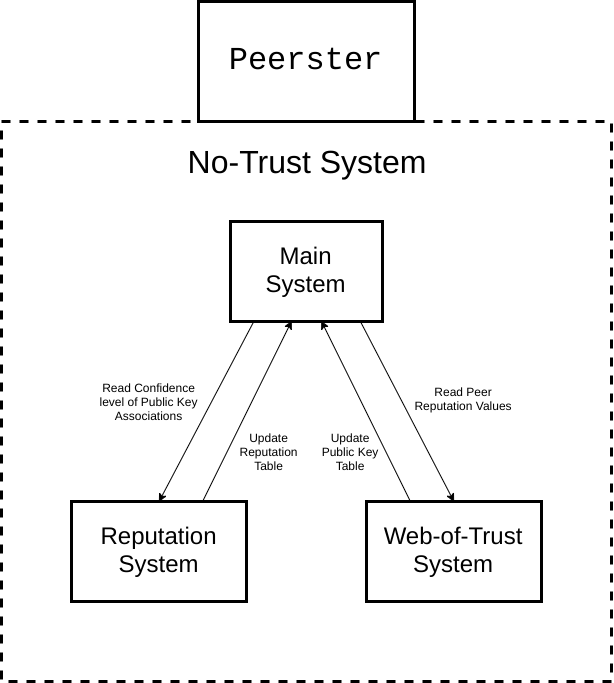
\includegraphics[width=50mm]{no-trust-arch}
	\centering
	\caption{General architecture of the No-Trust system}
	\label{fig:no-trust-arch}
\end{figure}

\subsection{Systems interoperability}

\subsubsection{Use of WTS for RS}

\subsubsection{Use of RS for WTS}
The reputation system will be useful for determining the probabilities as discussed in \ref{sec:parameters}, only the reputation corresponding to // TODO

\subsubsection{Use of WTS for the cryptographic functionalities}
This is quite evident. The WTS will provide the public keys needed for encryption and verification of signatures.

\section{Evaluation Plan}

\subsection{Cryptography}
\label{sec:crypt-test}
We will verify correctness of the cryptographic functionnalities (confidentiality, integrity and authentication) with some cases (e.g. sending well/badly signed files, sending encrypted messages and decoding them at receiver, ...), only to check that the standard libraries have been well implemented in our project. We will not evaluate the "crypto" and "crypto/rsa" libraries and will expect them to be correct.

\subsection{Web of Trust}
To measure the correctness and performance of our key distribution system (WTS), we will create a scenario with a network of Peerster nodes, and follow the updates of the key ring of each node, checking the time at which the ring stops updating, and checking the correctness of the ring. The state of the WTS system is the key ring, therefore checking the key ring is enough to evaluate the correctness of the system. The performance will be tested, but because of the nature of Peerster and the possibility of network bottlenecks, we will check that the key ring is complete after a reasonable amount of time. Moreover since the public keys are obtained via this system, testing in \ref{sec:crypt-test} will effectively test if the WTS works.

\bibliography{references}{}
\bibliographystyle{plain}

\end{document}
